\documentclass[a4paper,12pt]{article}
\usepackage{float}
\usepackage[table]{xcolor} % Para colorir as linhas da tabela
\usepackage{array} % Para melhorar a formatação de tabelas
\usepackage[brazil]{babel}
\usepackage[utf8]{inputenc}
\usepackage{indentfirst}
\usepackage{amsmath}
\usepackage{multicol}
\usepackage{graphicx}
\usepackage{animate}
\usepackage[font=footnotesize, labelfont=bf, listformat=empty]{caption}
\usepackage{geometry}
\usepackage{listings}
\usepackage{lastpage}
\usepackage{subcaption}
\usepackage[skins,xparse,breakable]{tcolorbox}
\usepackage{longtable}
\usepackage{minted}
\usepackage{titlesec}
\usepackage{fancyhdr}
\usepackage{setspace}
\usepackage[colorlinks=true, allcolors=black]{hyperref}

% Configurações de margens e espaçamento
\geometry{a4paper, left=2.5cm, right=2.5cm, top=2.5cm, bottom=2cm}
\setlength{\parindent}{1.25cm}
\onehalfspacing

% Configurações de títulos
\titleformat{\section}{\normalfont\large\bfseries}{\thesection}{1em}{}
\titleformat{\subsection}{\normalfont\bfseries}{\thesubsection}{1em}{}
\titleformat{\subsubsection}{\normalfont\itshape}{\thesubsubsection}{1em}{}

% Configurações de listagens
\renewcommand{\listingscaption}{Código}
\newenvironment{code}{\captionsetup{type=listing}}{}

% Configurações de cores
\definecolor{LightSeaGreen}{rgb}{0.1255, 0.6980, 0.6667}
\definecolor{whitesmoke}{rgb}{0.96, 0.96, 0.96}
\definecolor{cinza}{RGB}{160, 160, 160}
\definecolor{cinza_claro}{RGB}{240, 240, 240} % Cinza claro

% Configurações do minted para VHDL
\setminted[VHDL]{
    fontsize=\footnotesize,
    style=vs,
    linenos=true,
    breaklines=true,
    mathescape=true,
    bgcolor=cinza_claro,
    breakanywhere=true,
}

\newcommand{\hex}[1]{\textcolor{green!50!black}{#1}}

% Configurações de cabeçalho e rodapé
\pagestyle{fancy}
\fancyhf{}
\fancyhead[L]{\footnotesize{Laboratório de Sistemas Digitais - ENE0040}}
\fancyhead[R]{\footnotesize{2025/1 - Turma 07}}
\fancyfoot[R]{\footnotesize{Página \ \thepage \ de \pageref{LastPage}}}
\fancyfoot[L]{\footnotesize{Relatório do Experimento 3}}

% Adiciona uma linha preta acima do rodapé
\renewcommand{\footrulewidth}{0.4pt} % Espessura da linha
\renewcommand{\footrule}{\vbox to 0pt{\hrule width \textwidth height \footrulewidth \vss}} % Desenha a linha

% Novo Comando para chamar a capa
\newcommand{\capa}{
    \begin{titlepage}
        \begin{multicols}{2}
            \begin{flushleft}
                
\includegraphics[width=0.45\linewidth]{Recursos/Imagens/UnB_logo.png}
            \end{flushleft}
            \columnbreak
            \begin{flushright}
                Universidade de Brasília \\
                Faculdade de Tecnologia \\
                Departamento de Engenharia Elétrica
            \end{flushright}
        \end{multicols}
        \begin{center}
        \vspace{-20pt}
        \rule{\textwidth}{0.4pt}
        \end{center}
        \vspace{0.6cm}
        \begin{center}
            {\Huge \textbf{Relatório do Experimento 3}} \\[1em]
            {\large \textbf{Autor:} Henrique Morcelles Salum} \\[0.5em]
            {\large \textbf{Matrícula:} 232003008} \\
            \vfill
            {\large \textbf{ENE0040 - Laboratório de Sistemas Digitais - Turma 07}} \\
        \end{center}
    \end{titlepage}
}

\begin{document}

\capa

% Sumário
\newpage
\tableofcontents
\newpage

% Introdução
\section{Introdução}

\subsection{Sobre o Experimento}
\paragraph{}
Este experimento é composto por duas tarefas, em ambas, deve-se implementar circuitos lógicos com VHDL e simulá-los por meio do software ModelSim, da Intel. As especificidades de cada tarefa serão exploradas a seguir.

\subsubsection{Multiplexador 8 para 1}
\paragraph{}
Na primeira tarefa, devemos escrever, utilizando atribuições condicionais \textit{when-else}, uma entidade com dois vetores de entrada $S$, de três bits, e $D$, de oito bits, e um sinal de saída $Y$ que descreva um Mux 8x1. A tabela-verdade do sistema é a que segue:

\begin{table}[H]
    \footnotesize
    \centering
    \begin{tabular}{|c|c|c|c|}
        \hline
        \rowcolor{black}
        \textcolor{white}{$S_2$} & \textcolor{white}{$S_1$} & \textcolor{white}{$S_0$} & \textcolor{white}{Saída} \\ \hline
        0 & 0 & 0 & $D_0$ \\ \hline
        \rowcolor{cinza}
        0 & 0 & 1 & $D_1$ \\ \hline
        0 & 1 & 0 & $D_2$ \\ \hline
        \rowcolor{cinza}
        0 & 1 & 1 & $D_3$ \\ \hline
        1 & 0 & 0 & $D_4$ \\ \hline
        \rowcolor{cinza}
        1 & 0 & 1 & $D_5$ \\ \hline
        1 & 1 & 0 & $D_6$ \\ \hline
        \rowcolor{cinza}
        1 & 1 & 1 & $D_7$ \\ \hline
    \end{tabular}
    \caption{Tabela-verdade do multiplexador 8x1}
    \vspace{-5pt}
\end{table}


\subsubsection{Decodificador 4 para 16}
\paragraph{}
Na segunda tarefa, a entidade que devemos implementar em VHDL, utilizando atribuições seletivas \textit{with-select}, é um decodificador 4 para 16. Ele tem um vetor de entrada $A$, de quatro bits, e um vetor de saída $Y$, de 16 bits. A tabela-verdade é a que segue:

\begin{table}[H]
    \centering
    \footnotesize
    \setlength{\tabcolsep}{3pt}
    \begin{tabular}{|cccc|cccccccccccccccc|c|}
        \hline
        \rowcolor{black}
        \multicolumn{4}{|c|}{\textbf{\textcolor{white}{Entrada}}} & \multicolumn{17}{|c|}{\textbf{\textcolor{white}{Saída}}} \\ \hline
        \rowcolor{black}
        \textcolor{white}{$A_3$} & \textcolor{white}{$A_2$} & \textcolor{white}{$A_1$} & \textcolor{white}{$A_0$} & \textcolor{white}{$Y_{15}$} & \textcolor{white}{$Y_{14}$} & \textcolor{white}{$Y_{13}$} & \textcolor{white}{$Y_{12}$} & \textcolor{white}{$Y_{11}$} & \textcolor{white}{$Y_{10}$} & \textcolor{white}{$Y_9$} & \textcolor{white}{$Y_8$} & \textcolor{white}{$Y_7$} & \textcolor{white}{$Y_6$} & \textcolor{white}{$Y_5$} & \textcolor{white}{$Y_4$} & \textcolor{white}{$Y_3$} & \textcolor{white}{$Y_2$} & \textcolor{white}{$Y_1$} & \textcolor{white}{$Y_0$} & \textbf{\textcolor{white}{Hex}} \\ \hline
        0 & 0 & 0 & 0 & 0 & 0 & 0 & 0 &  0 & 0 & 0 & 0 & 0 & 0 & 0 & 0 &  0 & 0 & 0 & 1 & $0001h$ \\ \hline
        \rowcolor{cinza}
        0 & 0 & 0 & 1 & 0 & 0 & 0 & 0 & 0 & 0 & 0 & 0 & 0 & 0 & 0 & 0 & 0 & 0 & 1 & 0 & $0002h$ \\ \hline
        0 & 0 & 1 & 0 & 0 & 0 & 0 & 0 & 0 & 0 & 0 & 0 & 0 & 0 & 0 & 0 & 0 & 1 & 0 & 0 & $0004h$ \\ \hline
        \rowcolor{cinza}
        0 & 0 & 1 & 1 & 0 & 0 & 0 & 0 & 0 & 0 & 0 & 0 & 0 & 0 & 0 & 0 & 1 & 0 & 0 & 0 & $0008h$ \\ \hline
        0 & 1 & 0 & 0 & 0 & 0 & 0 & 0 & 0 & 0 & 0 & 0 & 0 & 0 & 0 & 1 & 0 & 0 & 0 & 0 & $0010h$ \\ \hline
        \rowcolor{cinza}
        0 & 1 & 0 & 1 & 0 & 0 & 0 & 0 & 0 & 0 & 0 & 0 & 0 & 0 & 1 & 0 & 0 & 0 & 0 & 0 & $0020h$ \\ \hline
        0 & 1 & 1 & 0 & 0 & 0 & 0 & 0 & 0 & 0 & 0 & 0 & 0 & 1 & 0 & 0 & 0 & 0 & 0 & 0 & $0040h$ \\ \hline
        \rowcolor{cinza}
        0 & 1 & 1 & 1 & 0 & 0 & 0 & 0 & 0 & 0 & 0 & 0 & 1 & 0 & 0 & 0 & 0 & 0 & 0 & 0 & $0080h$ \\ \hline
        1 & 0 & 0 & 0 & 0 & 0 & 0 & 0 & 0 & 0 & 0 & 1 & 0 & 0 & 0 & 0 & 0 & 0 & 0 & 0 & $0100h$ \\ \hline
        \rowcolor{cinza}
        1 & 0 & 0 & 1 & 0 & 0 & 0 & 0 & 0 & 0 & 1 & 0 & 0 & 0 & 0 & 0 & 0 & 0 & 0 & 0 & $0200h$ \\ \hline
        1 & 0 & 1 & 0 & 0 & 0 & 0 & 0 & 0 & 1 & 0 & 0 & 0 & 0 & 0 & 0 & 0 & 0 & 0 & 0 & $0400h$ \\ \hline
        \rowcolor{cinza}
        1 & 0 & 1 & 1 & 0 & 0 & 0 & 0 & 1 & 0 & 0 & 0 & 0 & 0 & 0 & 0 & 0 & 0 & 0 & 0 & $0800h$ \\ \hline
        1 & 1 & 0 & 0 & 0 & 0 & 0 & 1 & 0 & 0 & 0 & 0 & 0 & 0 & 0 & 0 & 0 & 0 & 0 & 0 & $1000h$ \\ \hline
        \rowcolor{cinza}
        1 & 1 & 0 & 1 & 0 & 0 & 1 & 0 & 0 & 0 & 0 & 0 & 0 & 0 & 0 & 0 & 0 & 0 & 0 & 0 & $2000h$ \\ \hline
        1 & 1 & 1 & 0 & 0 & 1 & 0 & 0 & 0 & 0 & 0 & 0 & 0 & 0 & 0 & 0 & 0 & 0 & 0 & 0 & $4000h$ \\ \hline
        \rowcolor{cinza}
        1 & 1 & 1 & 1 & 1 & 0 & 0 & 0 & 0 & 0 & 0 & 0 & 0 & 0 & 0 & 0 & 0 & 0 & 0 & 0 & $8000h$ \\ \hline
    \end{tabular}
    \caption{Tabela-verdade do Decodificador 4 para 16} \label{tab:dec4x16}
    \label{tab:dec4x16}
    \vspace{-20pt}
\end{table}

\paragraph{}
Note que, na \autoref{tab:dec4x16}, há uma coluna para a representação em hexadecimal da saída. Quando lidamos com representações binárias muito grandes, é conveniente utilizar essa representação pois, se um número em sua representação binária tem $n$ casas, em sua representação hexadecimal ele terá $log_2 n$. Além disso, a conversão de binário para hexadecimal é muito fácil: cada algarismo da representação hexadecimal é substituído pela sua representação binária - que tem quatro bits, já que o algarismo hexadecimal de maior valor é o $F_{16}$, que tem valor $15_{10} = 1111_{2}$ - e pronto! Representações hexadecimais serão utilizadas nos códigos em VHDL neste experimento.

\subsection{Introdução Teórica}

\subsubsection{Multiplexador 8 para 1}
\paragraph{}
Um multiplexador, também chamado de Mux, é um dispositivo digital que seleciona uma entre várias entradas de dados como saída. Essencialmente, o multiplexador atua como um ``comutador'' controlado por entradas de seleção, determinando qual sinal será encaminhado para a saída. Esse dispositivo é extensivamente usado no projeto de máquinas de estados, pois ele é muito conveniente quando é necessário implementar diferentes lógicas a depender do estado atual.

\paragraph{}
Para entender esse dispositivo, podemos separar as entradas entre entradas de dados, que são informações a serem selecionadas, e as entradas de seleção, que são utilizadas para escolher qual das entradas de dados será enviada para a saída. O número de entradas de seleção pode ser calculado em função do número de entradas de dados $n$ pela função:
\[
f(n) = \lceil \log_2n \rceil
\]

\paragraph{}
Nesse experimento, implementamos, especificamente, um multiplexador 8 para 1, ou seja, um multiplexador com oito entradas de dados e, consequentemente, $\log_2 8 = 3$ entradas de seleção, além de um sinal de saída.

\begin{figure}[H]
    \centering
    \scalebox{0.85}{
\begin{tikzpicture}[x=1pt,y=-1pt,line cap=rect]
\useasboundingbox (0,0) rectangle (135,165);
\definecolor{custcol_0_0_0}{RGB}{0, 0, 0}
\definecolor{custcol_ff_ff_ff}{RGB}{255, 255, 255}
\draw [line width=3.0pt, custcol_0_0_0 ]  (55.0,175.0) -- (55.0,195.0) ;
\draw [line width=3.0pt, custcol_0_0_0 ]  (75.0,165.0) -- (75.0,195.0) ;
\draw [line width=3.0pt, custcol_0_0_0 ]  (5.0,25.0) -- (35.0,25.0) ;
\draw [line width=3.0pt, custcol_0_0_0 ]  (5.0,45.0) -- (35.0,45.0) ;
\draw [line width=3.0pt, custcol_0_0_0 ]  (5.0,65.0) -- (35.0,65.0) ;
\draw [line width=3.0pt, custcol_0_0_0 ]  (5.0,85.0) -- (35.0,85.0) ;
\draw [line width=3.0pt, custcol_0_0_0 ]  (5.0,105.0) -- (35.0,105.0) ;
\draw [line width=3.0pt, custcol_0_0_0 ]  (5.0,125.0) -- (35.0,125.0) ;
\draw [line width=3.0pt, custcol_0_0_0 ]  (5.0,145.0) -- (35.0,145.0) ;
\draw [line width=3.0pt, custcol_0_0_0 ]  (5.0,165.0) -- (35.0,165.0) ;
\draw [line width=3.0pt, custcol_0_0_0 ]  (115.0,95.0) -- (135.0,95.0) ;
\draw [line width=3.0pt, custcol_0_0_0 ]  (95.0,155.0) -- (95.0,195.0) ;
\draw [line width=5.0pt, custcol_0_0_0 ]  (35.0,5.0) -- (35.0,186.0) -- (115.0,145.0) -- (115.0,46.0) -- cycle;
\fontsize{14pt}{14pt}\fontseries{bx}\sffamily\selectfont\node[inner sep=0, outer sep=0, custcol_0_0_0, anchor=base west] at  (42.5,30.0)  {0};
\fontsize{12pt}{12pt}\fontseries{bx}\sffamily\selectfont\node[inner sep=0, outer sep=0, custcol_0_0_0, anchor=base west] at  (50.0,165.0)  {S$_2$};
\fontsize{12pt}{12pt}\fontseries{bx}\sffamily\selectfont\node[inner sep=0, outer sep=0, custcol_0_0_0, anchor=base west] at  (69.0,155.0)  {S$_1$};
\fontsize{12pt}{12pt}\fontseries{bx}\sffamily\selectfont\node[inner sep=0, outer sep=0, custcol_0_0_0, anchor=base west] at  (88.0,145.0)  {S$_0$};
\fontsize{12pt}{12pt}\fontseries{bx}\sffamily\selectfont\node[inner sep=0, outer sep=0, custcol_0_0_0, anchor=base west] at  (98.0,99.0)  {Y};
\fill [line width=1.0pt, custcol_0_0_0]  (35.0,25.0) ellipse (2.0 and 2.0 );
\fill [line width=1.0pt, custcol_0_0_0]  (35.0,45.0) ellipse (2.0 and 2.0 );
\fill [line width=1.0pt, custcol_0_0_0]  (35.0,65.0) ellipse (2.0 and 2.0 );
\fill [line width=1.0pt, custcol_0_0_0]  (35.0,85.0) ellipse (2.0 and 2.0 );
\fill [line width=1.0pt, custcol_0_0_0]  (35.0,105.0) ellipse (2.0 and 2.0 );
\fill [line width=1.0pt, custcol_0_0_0]  (35.0,125.0) ellipse (2.0 and 2.0 );
\fill [line width=1.0pt, custcol_0_0_0]  (35.0,145.0) ellipse (2.0 and 2.0 );
\fill [line width=1.0pt, custcol_0_0_0]  (35.0,165.0) ellipse (2.0 and 2.0 );
\fill [line width=1.0pt, custcol_0_0_0]  (55.0,175.0) ellipse (2.0 and 2.0 );
\fill [line width=1.0pt, custcol_0_0_0]  (75.0,165.0) ellipse (2.0 and 2.0 );
\fill [line width=1.0pt, custcol_0_0_0]  (95.0,155.0) ellipse (2.0 and 2.0 );
\fill [line width=1.0pt, custcol_0_0_0]  (115.0,95.0) ellipse (2.0 and 2.0 );
\end{tikzpicture}
}
    \caption{Representação externa do multiplexador 8 x 1}
    \label{fig:Mux_externa}
\end{figure}

\subsubsection{Decodificador 4 para 16}
\paragraph{}
O decodificador, chamado de Dec, é um circuito combinatório com $n$ bits de entrada e $2^n$ bits de saída que, para cada combinação dos bits de entrada, ativa apenas um bit de saída. Por convenção, o bit ativado costuma estar na posição representada pelos bits de entrada. Nesse experimento, implementamos, especificamente, o Dec 4x16.

\begin{figure}[H]
    \centering
    % Important: If latex complains about unicode characters,
% please use "\usepackage[utf8x]{inputenc}" in your preamble
% You can change the size of the picture by putting it into the construct:
% 1) \resizebox{10cm}{!}{"below picture"} to scale horizontally to 10 cm
% 2) \resizebox{!}{15cm}{"below picture"} to scale vertically to 15 cm
% 3) \resizebox{10cm}{15cm}{"below picture"} a combination of above two
% It is not recomended to use the scale option of the tikzpicture environment.
\scalebox{0.85}{
\begin{tikzpicture}[x=1pt,y=-1pt,line cap=rect]
\useasboundingbox (0,0) rectangle (145,150);
\definecolor{custcol_0_0_0}{RGB}{0, 0, 0}
\definecolor{custcol_ff_ff_ff}{RGB}{255, 255, 255}
\draw [line width=3.0pt, custcol_0_0_0 ]  (125.0,47.0) -- (145.0,47.0) ;
\draw [line width=3.0pt, custcol_0_0_0 ]  (125.0,17.0) -- (145.0,17.0) ;
\draw [line width=3.0pt, custcol_0_0_0 ]  (125.0,27.0) -- (145.0,27.0) ;
\draw [line width=3.0pt, custcol_0_0_0 ]  (125.0,37.0) -- (145.0,37.0) ;
\draw [line width=3.0pt, custcol_0_0_0 ]  (125.0,57.0) -- (145.0,57.0) ;
\draw [line width=3.0pt, custcol_0_0_0 ]  (125.0,67.0) -- (145.0,67.0) ;
\draw [line width=3.0pt, custcol_0_0_0 ]  (125.0,77.0) -- (145.0,77.0) ;
\draw [line width=3.0pt, custcol_0_0_0 ]  (125.0,87.0) -- (145.0,87.0) ;
\draw [line width=3.0pt, custcol_0_0_0 ]  (125.0,97.0) -- (145.0,97.0) ;
\draw [line width=3.0pt, custcol_0_0_0 ]  (125.0,107.0) -- (145.0,107.0) ;
\draw [line width=3.0pt, custcol_0_0_0 ]  (125.0,117.0) -- (145.0,117.0) ;
\draw [line width=3.0pt, custcol_0_0_0 ]  (125.0,127.0) -- (145.0,127.0) ;
\draw [line width=3.0pt, custcol_0_0_0 ]  (125.0,137.0) -- (145.0,137.0) ;
\draw [line width=3.0pt, custcol_0_0_0 ]  (125.0,147.0) -- (145.0,147.0) ;
\draw [line width=3.0pt, custcol_0_0_0 ]  (125.0,157.0) -- (145.0,157.0) ;
\draw [line width=3.0pt, custcol_0_0_0 ]  (125.0,167.0) -- (145.0,167.0) ;
\draw [line width=3.0pt, custcol_0_0_0 ]  (5.0,17.0) -- (25.0,17.0) ;
\draw [line width=3.0pt, custcol_0_0_0 ]  (5.0,67.0) -- (25.0,67.0) ;
\draw [line width=3.0pt, custcol_0_0_0 ]  (5.0,117.0) -- (25.0,117.0) ;
\draw [line width=3.0pt, custcol_0_0_0 ]  (5.0,167.0) -- (25.0,167.0) ;
\draw [line width=5.0pt, custcol_0_0_0 ]  (25.0,7.0) -- (124.0,7.0) ;
\draw [line width=5.0pt, custcol_0_0_0 ]  (125.0,7.0) -- (125.0,176.0) ;
\draw [line width=5.0pt, custcol_0_0_0 ]  (125.0,177.0) -- (26.0,177.0) ;
\draw [line width=5.0pt, custcol_0_0_0 ]  (25.0,177.0) -- (25.0,8.0) ;
\fontsize{14pt}{14pt}\fontseries{bx}\sffamily\selectfont\node[inner sep=0, outer sep=0, custcol_0_0_0, anchor=base west] at  (109.0,23.0)  {\textbf{0}};
\fontsize{14pt}{14pt}\fontseries{bx}\sffamily\selectfont\node[inner sep=0, outer sep=0, custcol_0_0_0, anchor=base west] at  (31.0,122.0)  {A$_1$};
\fontsize{14pt}{14pt}\fontseries{bx}\sffamily\selectfont\node[inner sep=0, outer sep=0, custcol_0_0_0, anchor=base west] at  (32.0,170.0)  {A$_0$};
\fontsize{14pt}{14pt}\fontseries{bx}\sffamily\selectfont\node[inner sep=0, outer sep=0, custcol_0_0_0, anchor=base west] at  (32.0,73.0)  {A$_2$};
\fontsize{14pt}{14pt}\fontseries{bx}\sffamily\selectfont\node[inner sep=0, outer sep=0, custcol_0_0_0, anchor=base west] at  (32.0,25.0)  {A$_3$};
\fill [line width=1.0pt, custcol_0_0_0]  (25.0,17.0) ellipse (2.0 and 2.0 );
\fill [line width=1.0pt, custcol_0_0_0]  (25.0,67.0) ellipse (2.0 and 2.0 );
\fill [line width=1.0pt, custcol_0_0_0]  (25.0,117.0) ellipse (2.0 and 2.0 );
\fill [line width=1.0pt, custcol_0_0_0]  (25.0,167.0) ellipse (2.0 and 2.0 );
\fill [line width=1.0pt, custcol_0_0_0]  (125.0,17.0) ellipse (2.0 and 2.0 );
\fill [line width=1.0pt, custcol_0_0_0]  (125.0,27.0) ellipse (2.0 and 2.0 );
\fill [line width=1.0pt, custcol_0_0_0]  (125.0,37.0) ellipse (2.0 and 2.0 );
\fill [line width=1.0pt, custcol_0_0_0]  (125.0,47.0) ellipse (2.0 and 2.0 );
\fill [line width=1.0pt, custcol_0_0_0]  (125.0,57.0) ellipse (2.0 and 2.0 );
\fill [line width=1.0pt, custcol_0_0_0]  (125.0,67.0) ellipse (2.0 and 2.0 );
\fill [line width=1.0pt, custcol_0_0_0]  (125.0,77.0) ellipse (2.0 and 2.0 );
\fill [line width=1.0pt, custcol_0_0_0]  (125.0,87.0) ellipse (2.0 and 2.0 );
\fill [line width=1.0pt, custcol_0_0_0]  (125.0,97.0) ellipse (2.0 and 2.0 );
\fill [line width=1.0pt, custcol_0_0_0]  (125.0,107.0) ellipse (2.0 and 2.0 );
\fill [line width=1.0pt, custcol_0_0_0]  (125.0,117.0) ellipse (2.0 and 2.0 );
\fill [line width=1.0pt, custcol_0_0_0]  (125.0,127.0) ellipse (2.0 and 2.0 );
\fill [line width=1.0pt, custcol_0_0_0]  (125.0,137.0) ellipse (2.0 and 2.0 );
\fill [line width=1.0pt, custcol_0_0_0]  (125.0,147.0) ellipse (2.0 and 2.0 );
\fill [line width=1.0pt, custcol_0_0_0]  (125.0,157.0) ellipse (2.0 and 2.0 );
\fill [line width=1.0pt, custcol_0_0_0]  (125.0,167.0) ellipse (2.0 and 2.0 );
\end{tikzpicture}
}
    \caption{Representação externa do decodificador 4 x 16}
    \label{fig:dec4x16}
\end{figure}

\paragraph{}
Olhando para a \autoref{tab:dec4x16}, podemos perceber que cada saída do decodificador representa uma combinação dos $n$ bits de entrada, ou seja, um \textit{mintermo} dos bits de entrada. Esse fato justifica o interesse no decodificador: desde que toda função pode ser decomposta na soma dos mintermos que representam as linhas da tabela-verdade que essa função ativa, podemos fazer um $OR$ entre saídas específicas do Dec para gerar qualquer função booleana. Por exemplo:
\[
f(w, x, y, z) = \overline{w} \ \overline{x} \ \overline{y} \ \overline{z} + \overline{w} \ \overline{x} \ \overline{y} z + \overline{w} x \overline{y} \ \overline{z} + \overline{w}x \overline{y} z + \overline{w}xy\overline{z}
\]
\[
= \sum_{wxyz}m(0,1,4,5,6)
\]
Podemos implementar $f(w, x, y, z)$ da seguinte forma:

\begin{figure}[H]
    \centering
    % Important: If latex complains about unicode characters,
% please use "\usepackage[utf8x]{inputenc}" in your preamble
% You can change the size of the picture by putting it into the construct:
% 1) \resizebox{10cm}{!}{"below picture"} to scale horizontally to 10 cm
% 2) \resizebox{!}{15cm}{"below picture"} to scale vertically to 15 cm
% 3) \resizebox{10cm}{15cm}{"below picture"} a combination of above two
% It is not recomended to use the scale option of the tikzpicture environment.
\begin{tikzpicture}[x=1pt,y=-1pt,line cap=rect]
\useasboundingbox (0,0) rectangle (400,150);
\definecolor{custcol_0_0_0}{RGB}{0, 0, 0}
\definecolor{custcol_ff_ff_ff}{RGB}{255, 255, 255}
\draw [line width=3.0pt, custcol_0_0_0 ]  (319.0,40.0) -- (349.0,40.0) ;
\draw [line width=3.0pt, custcol_0_0_0 ]  (159.0,130.0) -- (179.0,130.0) ;
\draw [line width=3.0pt, custcol_0_0_0 ]  (159.0,90.0) -- (179.0,90.0) ;
\draw [line width=3.0pt, custcol_0_0_0 ]  (159.0,40.0) -- (179.0,40.0) ;
\draw [line width=3.0pt, custcol_0_0_0 ]  (159.0,50.0) -- (179.0,50.0) ;
\draw [line width=3.0pt, custcol_0_0_0 ]  (159.0,100.0) -- (179.0,100.0) ;
\draw [line width=3.0pt, custcol_0_0_0 ]  (159.0,110.0) -- (179.0,110.0) ;
\draw [line width=3.0pt, custcol_0_0_0 ]  (159.0,120.0) -- (179.0,120.0) ;
\draw [line width=3.0pt, custcol_0_0_0 ]  (159.0,140.0) -- (179.0,140.0) ;
\draw [line width=3.0pt, custcol_0_0_0 ]  (159.0,150.0) -- (179.0,150.0) ;
\draw [line width=3.0pt, custcol_0_0_0 ]  (159.0,160.0) -- (179.0,160.0) ;
\draw [line width=3.0pt, custcol_0_0_0 ]  (159.0,170.0) -- (179.0,170.0) ;
\draw [line width=3.0pt, custcol_0_0_0 ]  (39.0,20.0) -- (59.0,20.0) ;
\draw [line width=3.0pt, custcol_0_0_0 ]  (39.0,70.0) -- (59.0,70.0) ;
\draw [line width=3.0pt, custcol_0_0_0 ]  (39.0,120.0) -- (59.0,120.0) ;
\draw [line width=3.0pt, custcol_0_0_0 ]  (39.0,170.0) -- (59.0,170.0) ;
\draw [line width=5.0pt, custcol_0_0_0 ]  (59.0,10.0) -- (158.0,10.0) ;
\draw [line width=5.0pt, custcol_0_0_0 ]  (159.0,10.0) -- (159.0,179.0) ;
\draw [line width=5.0pt, custcol_0_0_0 ]  (159.0,180.0) -- (60.0,180.0) ;
\draw [line width=5.0pt, custcol_0_0_0 ]  (59.0,180.0) -- (59.0,11.0) ;
\fontsize{12pt}{12pt}\fontseries{bx}\sffamily\selectfont\node[inner sep=0, outer sep=0, custcol_0_0_0, anchor=base west] at  (145.0,25.0)  {0};
\fontsize{12pt}{12pt}\fontseries{bx}\sffamily\selectfont\node[inner sep=0, outer sep=0, custcol_0_0_0, anchor=base west] at  (65.0,125.0)  {A$_1$};
\fontsize{12pt}{12pt}\fontseries{bx}\sffamily\selectfont\node[inner sep=0, outer sep=0, custcol_0_0_0, anchor=base west] at  (65.0,175.0)  {A$_0$};
\fontsize{12pt}{12pt}\fontseries{bx}\sffamily\selectfont\node[inner sep=0, outer sep=0, custcol_0_0_0, anchor=base west] at  (65.0,75.0)  {A$_2$};
\fontsize{12pt}{12pt}\fontseries{bx}\sffamily\selectfont\node[inner sep=0, outer sep=0, custcol_0_0_0, anchor=base west] at  (65.0,25.0)  {A$_3$};
\fill [line width=1.0pt, custcol_0_0_0]  (59.0,20.0) ellipse (2.0 and 2.0 );
\fill [line width=1.0pt, custcol_0_0_0]  (59.0,70.0) ellipse (2.0 and 2.0 );
\fill [line width=1.0pt, custcol_0_0_0]  (59.0,120.0) ellipse (2.0 and 2.0 );
\fill [line width=1.0pt, custcol_0_0_0]  (59.0,170.0) ellipse (2.0 and 2.0 );
\fill [line width=1.0pt, custcol_0_0_0]  (159.0,20.0) ellipse (2.0 and 2.0 );
\fill [line width=1.0pt, custcol_0_0_0]  (159.0,30.0) ellipse (2.0 and 2.0 );
\fill [line width=1.0pt, custcol_0_0_0]  (159.0,40.0) ellipse (2.0 and 2.0 );
\fill [line width=1.0pt, custcol_0_0_0]  (159.0,50.0) ellipse (2.0 and 2.0 );
\fill [line width=1.0pt, custcol_0_0_0]  (159.0,60.0) ellipse (2.0 and 2.0 );
\fill [line width=1.0pt, custcol_0_0_0]  (159.0,70.0) ellipse (2.0 and 2.0 );
\fill [line width=1.0pt, custcol_0_0_0]  (159.0,80.0) ellipse (2.0 and 2.0 );
\fill [line width=1.0pt, custcol_0_0_0]  (159.0,90.0) ellipse (2.0 and 2.0 );
\fill [line width=1.0pt, custcol_0_0_0]  (159.0,100.0) ellipse (2.0 and 2.0 );
\fill [line width=1.0pt, custcol_0_0_0]  (159.0,110.0) ellipse (2.0 and 2.0 );
\fill [line width=1.0pt, custcol_0_0_0]  (159.0,120.0) ellipse (2.0 and 2.0 );
\fill [line width=1.0pt, custcol_0_0_0]  (159.0,130.0) ellipse (2.0 and 2.0 );
\fill [line width=1.0pt, custcol_0_0_0]  (159.0,140.0) ellipse (2.0 and 2.0 );
\fill [line width=1.0pt, custcol_0_0_0]  (159.0,150.0) ellipse (2.0 and 2.0 );
\fill [line width=1.0pt, custcol_0_0_0]  (159.0,160.0) ellipse (2.0 and 2.0 );
\fill [line width=1.0pt, custcol_0_0_0]  (159.0,170.0) ellipse (2.0 and 2.0 );
\draw [line width=2.0pt, custcol_0_0_0 ]  (21.0,12.0) -- (38.0,12.0) ;
\draw [line width=2.0pt, custcol_0_0_0 ]  (39.0,12.0) -- (39.0,29.0) ;
\draw [line width=2.0pt, custcol_0_0_0 ]  (39.0,30.0) -- (22.0,30.0) ;
\draw [line width=2.0pt, custcol_0_0_0 ]  (21.0,30.0) -- (21.0,13.0) ;
\fontsize{12pt}{12pt}\selectfont\node[inner sep=0, outer sep=0, custcol_0_0_0, anchor=base west] at  (23.0,27.0)  {x1};
\fontsize{16pt}{16pt}\fontseries{bx}\selectfont\node[inner sep=0, outer sep=0, custcol_0_0_0, anchor=base west] at  (5.0,28.0)  {$w$};
\fill [line width=2.0pt, custcol_0_0_0]  (39.0,20.0) ellipse (2.0 and 2.0 );
\draw [line width=2.0pt, custcol_0_0_0 ]  (21.0,62.0) -- (38.0,62.0) ;
\draw [line width=2.0pt, custcol_0_0_0 ]  (39.0,62.0) -- (39.0,79.0) ;
\draw [line width=2.0pt, custcol_0_0_0 ]  (39.0,80.0) -- (22.0,80.0) ;
\draw [line width=2.0pt, custcol_0_0_0 ]  (21.0,80.0) -- (21.0,63.0) ;
\fontsize{12pt}{12pt}\selectfont\node[inner sep=0, outer sep=0, custcol_0_0_0, anchor=base west] at  (23.0,77.0)  {x1};
\fontsize{16pt}{16pt}\fontseries{bx}\selectfont\node[inner sep=0, outer sep=0, custcol_0_0_0, anchor=base west] at  (8.0,78.0)  {$x$};
\fill [line width=2.0pt, custcol_0_0_0]  (39.0,70.0) ellipse (2.0 and 2.0 );
\draw [line width=2.0pt, custcol_0_0_0 ]  (21.0,112.0) -- (38.0,112.0) ;
\draw [line width=2.0pt, custcol_0_0_0 ]  (39.0,112.0) -- (39.0,129.0) ;
\draw [line width=2.0pt, custcol_0_0_0 ]  (39.0,130.0) -- (22.0,130.0) ;
\draw [line width=2.0pt, custcol_0_0_0 ]  (21.0,130.0) -- (21.0,113.0) ;
\fontsize{12pt}{12pt}\selectfont\node[inner sep=0, outer sep=0, custcol_0_0_0, anchor=base west] at  (23.0,127.0)  {x1};
\fontsize{16pt}{16pt}\fontseries{bx}\selectfont\node[inner sep=0, outer sep=0, custcol_0_0_0, anchor=base west] at  (8.0,128.0)  {$y$};
\fill [line width=2.0pt, custcol_0_0_0]  (39.0,120.0) ellipse (2.0 and 2.0 );
\draw [line width=2.0pt, custcol_0_0_0 ]  (21.0,162.0) -- (38.0,162.0) ;
\draw [line width=2.0pt, custcol_0_0_0 ]  (39.0,162.0) -- (39.0,179.0) ;
\draw [line width=2.0pt, custcol_0_0_0 ]  (39.0,180.0) -- (22.0,180.0) ;
\draw [line width=2.0pt, custcol_0_0_0 ]  (21.0,180.0) -- (21.0,163.0) ;
\fontsize{12pt}{12pt}\selectfont\node[inner sep=0, outer sep=0, custcol_0_0_0, anchor=base west] at  (23.0,177.0)  {x1};
\fontsize{16pt}{16pt}\fontseries{bx}\selectfont\node[inner sep=0, outer sep=0, custcol_0_0_0, anchor=base west] at  (9.0,178.0)  {$z$};
\fill [line width=2.0pt, custcol_0_0_0]  (39.0,170.0) ellipse (2.0 and 2.0 );
\draw [line width=3.0pt, custcol_0_0_0 ]  (159.0,20.0) -- (269.0,20.0) -- (269.0,20.0) ;
\draw [line width=3.0pt, custcol_0_0_0 ]  (159.0,30.0) -- (269.0,30.0) -- (274.0,30.0) ;
\draw [line width=3.0pt, custcol_0_0_0 ]  (159.0,60.0) -- (219.0,60.0) -- (219.0,40.0) -- (269.0,40.0) -- (275.0,40.0) ;
\draw [line width=3.0pt, custcol_0_0_0 ]  (159.0,70.0) -- (229.0,70.0) -- (229.0,50.0) -- (269.0,50.0) -- (274.0,50.0) ;
\draw [line width=3.0pt, custcol_0_0_0 ]  (159.0,80.0) -- (239.0,80.0) -- (239.0,60.0) -- (269.0,60.0) -- (271.0,60.0) ;
\draw [line width=2.0pt, custcol_0_0_0 ]  (319.0,40.0) .. controls  (299.0,15.0)  ..  (269.0,15.0) .. controls  (282.0,40.0)  ..  (269.0,65.0) .. controls  (299.0,65.0)  ..  (319.0,40.0) -- cycle ;
\draw [line width=2.0pt, custcol_0_0_0]  (360.0,41.0) ellipse (9.0 and 9.0 );
\fontsize{12pt}{12pt}\selectfont\node[inner sep=0, outer sep=0, custcol_0_0_0, anchor=base west] at  (353.0,47.0)  {x1};
\fill [line width=2.0pt, custcol_0_0_0]  (349.0,40.0) ellipse (2.0 and 2.0 );
\fontsize{14pt}{14pt}\selectfont\node[inner sep=0, outer sep=0, custcol_0_0_0, anchor=base west] at  (335.0,22.0)  {$f(w,x,y,z)$};
\end{tikzpicture}


    \label{fig:enter-label}
\end{figure}


\section{Códigos}
\paragraph{}
Nessa seção, serão apresentados os códigos desenvolvidos, em VHDL, para implementar os sistemas digitais apresentados na introdução. Aqui, alguns comentários foram suprimidos para melhor apresentação, mas os códigos enviados junto a este relatório estão todos devidamente comentados.

\subsection{Multiplexador 8 para 1}

\subsubsection{Descrição de Hardware}
\paragraph{}
O código escrito para implementar o modelo de \textit{hardware} do Mux 8x1, utilizando atribuições condicionais \textit{when-else} está exibido abaixo.

\begin{code}
\begin{minted}{VHDL}
library IEEE;
use IEEE.std_logic_1164.all;

entity Mux8x1 is
    port (
        D: in std_logic_vector(7 downto 0);
        S: in std_logic_vector(2 downto 0);
        Y: out std_logic
    );
end entity Mux8x1;

architecture behavioral of Mux8x1 is
begin
    Y <= D(7) when (S = "111") else
         D(6) when (S = "110") else
         D(5) when (S = "101") else
         D(4) when (S = "100") else
         D(3) when (S = "011") else
         D(2) when (S = "010") else
         D(1) when (S = "001") else
         D(0) when (S = "000") else
         '-';    
end architecture behavioral;
\end{minted}
\caption{Código de \textit{design} do multiplexador 8 para 1}
\end{code}

\subsubsection{Testbench}
\paragraph{}
Além do código acima, foi necessário implementar, também em VHDL, um \textit{testbench} para que se pudesse testar o comportamento e a funcionalidade do circuito digital projetado. Com ele, podemos gerar todas as combinações de interesse dos sinais de entrada e analisar o comportamento do circuito sob cada um desses estímulos. O código para implementar esse \textit{testbench} é o que segue:

\begin{code}
\begin{minted}{VHDL}
library IEEE;
use IEEE.std_logic_1164.all;
use ieee.numeric_std.all;

entity tb_Mux8x1 is
end entity tb_Mux8x1;

architecture main of tb_Mux8x1 is
    component Mux8x1 is
        port (
            D: in std_logic_vector(7 downto 0);
            S: in std_logic_vector(2 downto 0);
            Y: out std_logic
        );
    end component Mux8x1;
    signal D_tb: std_logic_vector(7 downto 0) := (others => '1');
    signal S_tb: std_logic_vector(2 downto 0) := (others => '0');
begin
    instancia_Mux8x1: component Mux8x1
        port map (
            D => D_tb,
            S => S_tb,
            Y => open
        );
    -- Processo para variar as entradas de seleção
    estimulos_seletoras: process
        variable s_unsigned: unsigned(2 downto 0);
    begin
        wait for 12.5 ns;
        s_unsigned := unsigned(S_tb);
        s_unsigned := s_unsigned + 1;
        S_tb <= std_logic_vector(s_unsigned);
    end process estimulos_seletoras;
    -- Processo para variar as entradas selecionadas
    variacao_dados: process
        variable i: integer;
    begin
        wait for 6.25 ns;
        i := to_integer(unsigned(S_tb));
        D_tb(i) <= not D_tb(i);
        wait on S_tb;
    end process variacao_dados;
end architecture main;
\end{minted}
\caption{Testbench do multiplexador 8 para 1}
\label{cod:testbench_mux}
\end{code}

\paragraph{}
No código acima, o multiplexador construído é instanciado e utilizado como uma ``caixa-preta''; associamos às suas entradas sinais do \textit{testbench}, o que é equivalente a conectar cabos nas entradas de um dispositivo digital, e, dentro do \textit{process}, fazemos esses sinais oscilarem. Dessa forma, conseguimos testar o dispositivo criado.

\subsection{Decodificador 4 para 16}
\subsubsection{Descrição de \textit{Hardware}}
\paragraph{}
O código, em VHDL, que descreve o circuito do decodificador 4 para 16, utilizando atribuição seletiva \textit{with-select}, é o que segue:

\begin{code}
\begin{minted}[escapeinside=||]{VHDL}
library IEEE;
use IEEE.std_logic_1164.all;

entity Dec4x16 is
    port (
        A: in std_logic_vector(3 downto 0);
        Y: out std_logic_vector(15 downto 0)
    );
end entity Dec4x16;

architecture behavioral of Dec4x16 is
begin
    with A select Y <=
        |\hex{X"0001"}| when |\hex{X"0"}|,
        |\hex{X"0002"}| when |\hex{X"1"}|,
        |\hex{X"0004"}| when |\hex{X"2"}|,
        |\hex{X"0008"}| when |\hex{X"3"}|,
        |\hex{X"0010"}| when |\hex{X"4"}|,
        |\hex{X"0020"}| when |\hex{X"5"}|,
        |\hex{X"0040"}| when |\hex{X"6"}|,
        |\hex{X"0080"}| when |\hex{X"7"}|,
        |\hex{X"0100"}| when |\hex{X"8"}|,
        |\hex{X"0200"}| when |\hex{X"9"}|,
        |\hex{X"0400"}| when |\hex{X"A"}|,
        |\hex{X"0800"}| when |\hex{X"B"}|,
        |\hex{X"1000"}| when |\hex{X"C"}|,
        |\hex{X"2000"}| when |\hex{X"D"}|,
        |\hex{X"4000"}| when |\hex{X"E"}|,
        |\hex{X"8000"}| when |\hex{X"F"}|,
        "----------------" when others;
end architecture behavioral;
\end{minted}
\vspace{-20pt}
\caption{Código para implementação do decodificador 4x16}
\vspace{-10pt}
\end{code}

\paragraph{}
Nesse código, utilizamos o VHDL em alto nível, com a abstração \textit{with-select}. Além disso, representamos os vetores de bits por hexadecimais, precedidos por `X' no VHDL.

\subsubsection{Testbench}
\paragraph{}
Assim como com o multiplexador, precisamos fazer um \textit{testbench} para o decodificador para testarmos o dispositivo implementado. O código desse \textit{testbench} está exibido a seguir.

\begin{code}
\begin{minted}{VHDL}
library IEEE;
use IEEE.std_logic_1164.all;
use IEEE.numeric_std.all;

entity tb_Dec4x16 is
end entity tb_Dec4x16;

architecture testbench of tb_Dec4x16 is

    component Dec4x16 is
        port (
            A: in std_logic_vector(3 downto 0);
            Y: out std_logic_vector(15 downto 0)
        );
    end component Dec4x16;
    
    signal A_tb: std_logic_vector(3 downto 0) := (others => '0');
begin
    instancia_Dec4x16: component Dec4x16
        port map (
            A => A_tb,
            Y => open
        );

    estimulos: process
        variable Uns_A: unsigned(3 downto 0);
    begin
        wait for 6.25 ns;
        Uns_A := unsigned(A_tb);
        A_tb <= std_logic_vector(Uns_A + 1);
    end process estimulos;
end architecture testbench;
\end{minted}
\caption{Testbench para o decodificador 4x16}
\end{code}

\paragraph{}
No código acima, diferente do Código \autoref{cod:testbench_mux}, em que geramos apenas algumas combinações de interesse, geramos todas as combinações possíveis das entradas. Isso se deve à natureza do decodificador: diferente do multiplexador, todas as combinações possíveis das entradas são de interesse, pois todas interferem na saída a qualquer momento.

% Compilação
\section{Compilação}
\paragraph{}
Após escrever os códigos, é necessário compilá-los pelo ModelSim para que se possa simular os sistemas digitais discutidos. Caso a compilação tenha sucesso, sabemos que não houve erros nos códigos apresentados, mas ainda não podemos afirmar que a lógica para implementar os circuitos está correta; isso será analisado nas próximas seções. A seguir, está a mensagem de compilação dos códigos apresentados acima, sem nenhum erro, como pode ser visto no terminal no canto inferior da figura.

\begin{figure}[H]
    \centering
    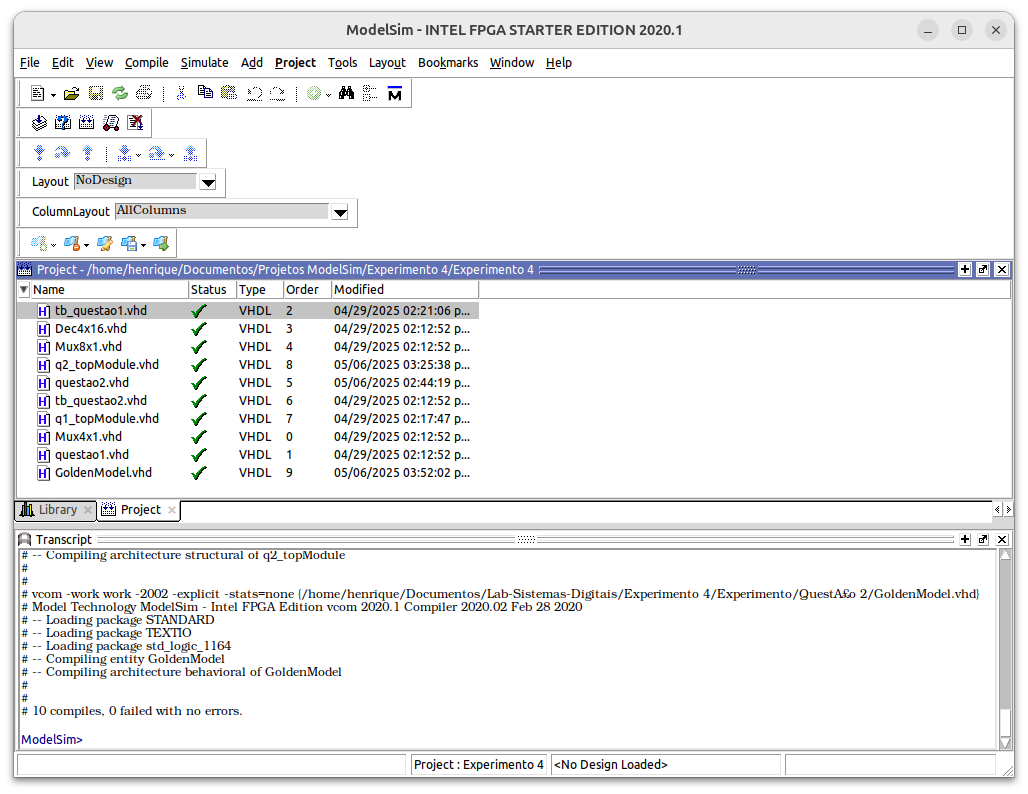
\includegraphics[width=1\textwidth]{Recursos/Imagens/CompileModelSim.png}
    \caption{Compilação de todos os códigos apresentados}
\end{figure}

\newpage

\section{Simulação}
\paragraph{}
Após compilar com sucesso os códigos apresentados, utilizamos o ModelSim para simular o comportamento dos sistemas descritos por eles. Lá, utilizamos a aba ``Waves'' para analisar o comportamento dos sinais de saída para cada combinação de valores dos sinais de entrada. A forma como as entradas variam segue o que definimos nos \textit{testbenches}, então note que as ondas referentes ao Mux 8x1 não representam todas as combinações das seis entradas. Seguem as imagens das simulações no ModelSim dos sistemas projetados.

\begin{figure}[H]
    \centering
    \begin{tcolorbox}[colframe=cinza, colback=white, boxrule=0.75pt, arc=0pt, width=1\textwidth, center, boxsep=0pt, left=0pt, right=0pt, top=0pt, bottom=0pt]
    \includegraphics[width=1\textwidth]{Recursos/Imagens/wave_mux8x1.png}
    \end{tcolorbox}
    \caption{Simulação em forma de onda binária do multiplexador 8 para 1}
\end{figure}

\begin{figure}[H]
    \centering
    \begin{tcolorbox}[colframe=cinza, colback=white, boxrule=0.75pt, arc=0pt, width=1\textwidth, center, boxsep=0pt, left=0pt, right=0pt, top=0pt, bottom=0pt]
    \includegraphics[width=1\textwidth]{Recursos/Imagens/wave_dec4x16.png}
    \end{tcolorbox}
    \caption{Simulação em forma de onda binária do decodificador 4 para 16}
\end{figure}

% Análise
\section{Análise}

\paragraph{}
Para analisar os resultados obtidos, basta olhar para os valores das ondas das entradas e saídas entre cada mudança dos sinais de entrada. Os cursores estão posicionados de forma que, ao selecionar cada um deles, vemos todas as possíveis combinações das entradas e saídas correspondentes na aba à esquerda da tela.

\subsection{Análise do comportamento do Multiplexador 8 para 1}
\paragraph{}
 Abaixo, exibimos os \textit{prints} que denotam o comportamento do sinal de saída $Y$ para cada combinação da entrada de seleção $S$ e selecionada $D_n$.

\setlength{\fboxsep}{0pt} % Espaçamento entre a borda e a imagem
\begin{figure}[H]
    \centering
    \fcolorbox{cinza}{white}{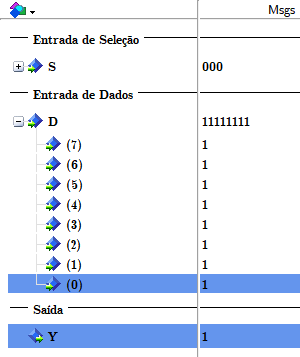
\includegraphics[width=0.21\textwidth]{Recursos/Imagens/011.png}}
    \fcolorbox{cinza}{white}{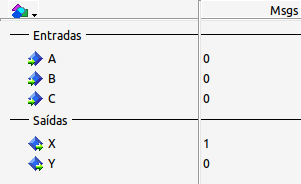
\includegraphics[width=0.21\textwidth]{Recursos/Imagens/000.png}}
    \fcolorbox{cinza}{white}{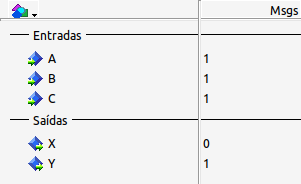
\includegraphics[width=0.21\textwidth]{Recursos/Imagens/111.png}}
    \fcolorbox{cinza}{white}{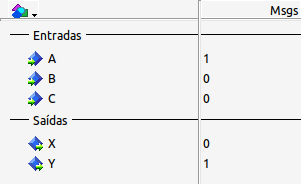
\includegraphics[width=0.21\textwidth]{Recursos/Imagens/100.png}} \\
    \fcolorbox{cinza}{white}{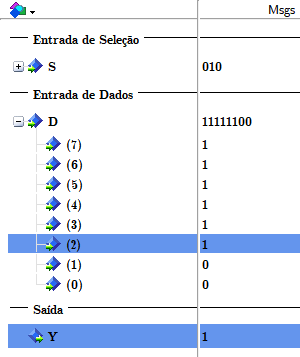
\includegraphics[width=0.21\textwidth]{Recursos/Imagens/211.png}}
    \fcolorbox{cinza}{white}{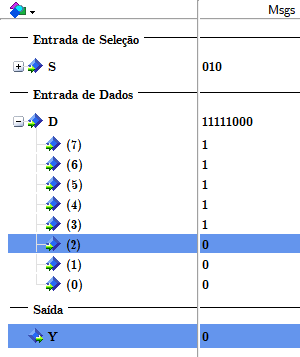
\includegraphics[width=0.21\textwidth]{Recursos/Imagens/200.png}}
    \fcolorbox{cinza}{white}{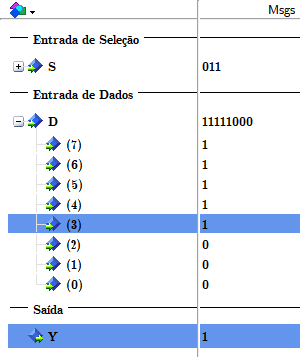
\includegraphics[width=0.21\textwidth]{Recursos/Imagens/311.png}}
    \fcolorbox{cinza}{white}{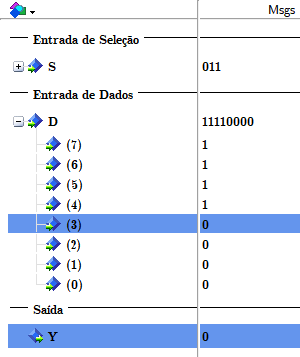
\includegraphics[width=0.21\textwidth]{Recursos/Imagens/300.png}} \\
    \fcolorbox{cinza}{white}{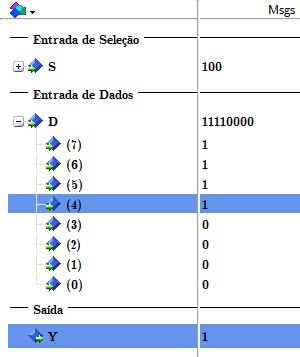
\includegraphics[width=0.21\textwidth]{Recursos/Imagens/411.png}}
    \fcolorbox{cinza}{white}{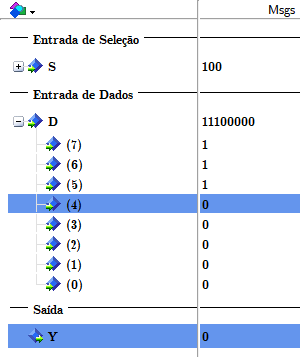
\includegraphics[width=0.21\textwidth]{Recursos/Imagens/400.png}}
    \fcolorbox{cinza}{white}{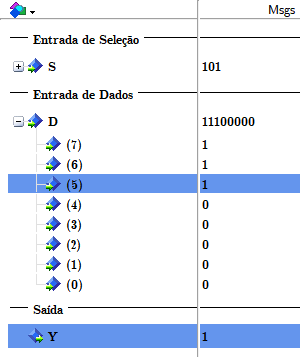
\includegraphics[width=0.21\textwidth]{Recursos/Imagens/511.png}}
    \fcolorbox{cinza}{white}{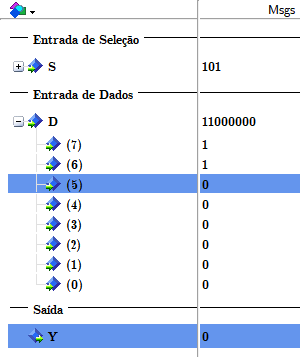
\includegraphics[width=0.21\textwidth]{Recursos/Imagens/500.png}} \\
    \fcolorbox{cinza}{white}{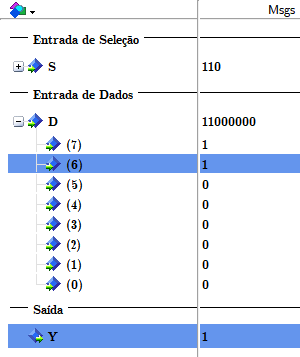
\includegraphics[width=0.21\textwidth]{Recursos/Imagens/611.png}}
    \fcolorbox{cinza}{white}{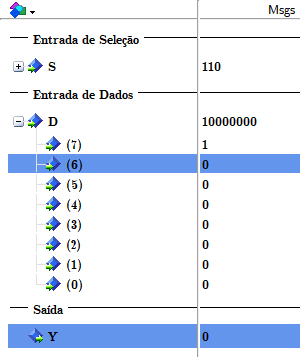
\includegraphics[width=0.21\textwidth]{Recursos/Imagens/600.png}}
    \fcolorbox{cinza}{white}{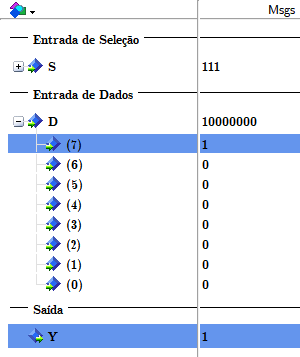
\includegraphics[width=0.21\textwidth]{Recursos/Imagens/711.png}}
    \fcolorbox{cinza}{white}{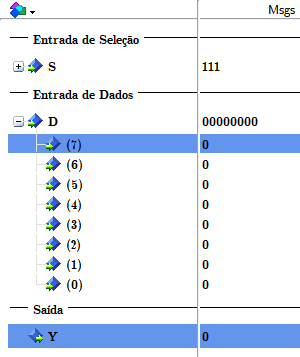
\includegraphics[width=0.21\textwidth]{Recursos/Imagens/700.png}}
    \caption{Combinações de entradas de seleção e saídas correspondentes do multiplexador 8 para 1}
    \vspace{-10pt}
\end{figure}

\paragraph{}
Percebe-se que o comportamento está de acordo com o esperado: quando a entrada de seleção seleciona a entrada de dados $D_n$, $Y=D_n$.

\subsection{Análise do comportamento do Decodificador 4 para 16}

\paragraph{}
Exibimos abaixo os \textit{prints} da seção à esquerda da aba waves do ModelSim para cada combinação possível da entrada.

\begin{figure}[H]
    \centering
    % Important: If latex complains about unicode characters,
% please use "\usepackage[utf8x]{inputenc}" in your preamble
% You can change the size of the picture by putting it into the construct:
% 1) \resizebox{10cm}{!}{"below picture"} to scale horizontally to 10 cm
% 2) \resizebox{!}{15cm}{"below picture"} to scale vertically to 15 cm
% 3) \resizebox{10cm}{15cm}{"below picture"} a combination of above two
% It is not recomended to use the scale option of the tikzpicture environment.
\scalebox{0.85}{
\begin{tikzpicture}[x=1pt,y=-1pt,line cap=rect]
\useasboundingbox (0,0) rectangle (145,150);
\definecolor{custcol_0_0_0}{RGB}{0, 0, 0}
\definecolor{custcol_ff_ff_ff}{RGB}{255, 255, 255}
\draw [line width=3.0pt, custcol_0_0_0 ]  (125.0,47.0) -- (145.0,47.0) ;
\draw [line width=3.0pt, custcol_0_0_0 ]  (125.0,17.0) -- (145.0,17.0) ;
\draw [line width=3.0pt, custcol_0_0_0 ]  (125.0,27.0) -- (145.0,27.0) ;
\draw [line width=3.0pt, custcol_0_0_0 ]  (125.0,37.0) -- (145.0,37.0) ;
\draw [line width=3.0pt, custcol_0_0_0 ]  (125.0,57.0) -- (145.0,57.0) ;
\draw [line width=3.0pt, custcol_0_0_0 ]  (125.0,67.0) -- (145.0,67.0) ;
\draw [line width=3.0pt, custcol_0_0_0 ]  (125.0,77.0) -- (145.0,77.0) ;
\draw [line width=3.0pt, custcol_0_0_0 ]  (125.0,87.0) -- (145.0,87.0) ;
\draw [line width=3.0pt, custcol_0_0_0 ]  (125.0,97.0) -- (145.0,97.0) ;
\draw [line width=3.0pt, custcol_0_0_0 ]  (125.0,107.0) -- (145.0,107.0) ;
\draw [line width=3.0pt, custcol_0_0_0 ]  (125.0,117.0) -- (145.0,117.0) ;
\draw [line width=3.0pt, custcol_0_0_0 ]  (125.0,127.0) -- (145.0,127.0) ;
\draw [line width=3.0pt, custcol_0_0_0 ]  (125.0,137.0) -- (145.0,137.0) ;
\draw [line width=3.0pt, custcol_0_0_0 ]  (125.0,147.0) -- (145.0,147.0) ;
\draw [line width=3.0pt, custcol_0_0_0 ]  (125.0,157.0) -- (145.0,157.0) ;
\draw [line width=3.0pt, custcol_0_0_0 ]  (125.0,167.0) -- (145.0,167.0) ;
\draw [line width=3.0pt, custcol_0_0_0 ]  (5.0,17.0) -- (25.0,17.0) ;
\draw [line width=3.0pt, custcol_0_0_0 ]  (5.0,67.0) -- (25.0,67.0) ;
\draw [line width=3.0pt, custcol_0_0_0 ]  (5.0,117.0) -- (25.0,117.0) ;
\draw [line width=3.0pt, custcol_0_0_0 ]  (5.0,167.0) -- (25.0,167.0) ;
\draw [line width=5.0pt, custcol_0_0_0 ]  (25.0,7.0) -- (124.0,7.0) ;
\draw [line width=5.0pt, custcol_0_0_0 ]  (125.0,7.0) -- (125.0,176.0) ;
\draw [line width=5.0pt, custcol_0_0_0 ]  (125.0,177.0) -- (26.0,177.0) ;
\draw [line width=5.0pt, custcol_0_0_0 ]  (25.0,177.0) -- (25.0,8.0) ;
\fontsize{14pt}{14pt}\fontseries{bx}\sffamily\selectfont\node[inner sep=0, outer sep=0, custcol_0_0_0, anchor=base west] at  (109.0,23.0)  {\textbf{0}};
\fontsize{14pt}{14pt}\fontseries{bx}\sffamily\selectfont\node[inner sep=0, outer sep=0, custcol_0_0_0, anchor=base west] at  (31.0,122.0)  {A$_1$};
\fontsize{14pt}{14pt}\fontseries{bx}\sffamily\selectfont\node[inner sep=0, outer sep=0, custcol_0_0_0, anchor=base west] at  (32.0,170.0)  {A$_0$};
\fontsize{14pt}{14pt}\fontseries{bx}\sffamily\selectfont\node[inner sep=0, outer sep=0, custcol_0_0_0, anchor=base west] at  (32.0,73.0)  {A$_2$};
\fontsize{14pt}{14pt}\fontseries{bx}\sffamily\selectfont\node[inner sep=0, outer sep=0, custcol_0_0_0, anchor=base west] at  (32.0,25.0)  {A$_3$};
\fill [line width=1.0pt, custcol_0_0_0]  (25.0,17.0) ellipse (2.0 and 2.0 );
\fill [line width=1.0pt, custcol_0_0_0]  (25.0,67.0) ellipse (2.0 and 2.0 );
\fill [line width=1.0pt, custcol_0_0_0]  (25.0,117.0) ellipse (2.0 and 2.0 );
\fill [line width=1.0pt, custcol_0_0_0]  (25.0,167.0) ellipse (2.0 and 2.0 );
\fill [line width=1.0pt, custcol_0_0_0]  (125.0,17.0) ellipse (2.0 and 2.0 );
\fill [line width=1.0pt, custcol_0_0_0]  (125.0,27.0) ellipse (2.0 and 2.0 );
\fill [line width=1.0pt, custcol_0_0_0]  (125.0,37.0) ellipse (2.0 and 2.0 );
\fill [line width=1.0pt, custcol_0_0_0]  (125.0,47.0) ellipse (2.0 and 2.0 );
\fill [line width=1.0pt, custcol_0_0_0]  (125.0,57.0) ellipse (2.0 and 2.0 );
\fill [line width=1.0pt, custcol_0_0_0]  (125.0,67.0) ellipse (2.0 and 2.0 );
\fill [line width=1.0pt, custcol_0_0_0]  (125.0,77.0) ellipse (2.0 and 2.0 );
\fill [line width=1.0pt, custcol_0_0_0]  (125.0,87.0) ellipse (2.0 and 2.0 );
\fill [line width=1.0pt, custcol_0_0_0]  (125.0,97.0) ellipse (2.0 and 2.0 );
\fill [line width=1.0pt, custcol_0_0_0]  (125.0,107.0) ellipse (2.0 and 2.0 );
\fill [line width=1.0pt, custcol_0_0_0]  (125.0,117.0) ellipse (2.0 and 2.0 );
\fill [line width=1.0pt, custcol_0_0_0]  (125.0,127.0) ellipse (2.0 and 2.0 );
\fill [line width=1.0pt, custcol_0_0_0]  (125.0,137.0) ellipse (2.0 and 2.0 );
\fill [line width=1.0pt, custcol_0_0_0]  (125.0,147.0) ellipse (2.0 and 2.0 );
\fill [line width=1.0pt, custcol_0_0_0]  (125.0,157.0) ellipse (2.0 and 2.0 );
\fill [line width=1.0pt, custcol_0_0_0]  (125.0,167.0) ellipse (2.0 and 2.0 );
\end{tikzpicture}
}
    \caption{Todas as combinações de entradas e as saídas correspondentes do decodificador 4 para 16}
    \vspace{-15pt}
\end{figure}

\paragraph{}
Novamente, percebe-se que o comportamento está de acordo com o esperado. Cada um dos \textit{prints} acima representa uma linha da tabela-verdade do decodificador 4 para 16 e, analisando-os, percebemos que a saída está de acordo com o exibido na \autoref{tab:dec4x16}.

\section{Conclusão}

\paragraph{}
Nesse experimento, simulou-se dois dispositivos digitais de suma importância para a eletrônica digital: o Multiplexador 8 para 1 e o decodificador 4 para 16.

\paragraph{}
Pelo relatório, concluímos o sucesso do experimento ao analisarmos devidamente os resultados obtidos pelas simulações: notamos que o comportamento dos sistemas explorados foi exatamente o esperado para todo possível estímulo, isto é, não foram observadas discrepâncias entre o comportamento esperado e o observado.

\end{document}